\hyperdef{}{tilda}{}

\subsection{\texorpdfstring{{Organisatorisches}}{Organisatorisches}}

\subsubsection{\texorpdfstring{{Zeiten}}{Zeiten}}

Die Sitzungen werden an vier Tagen jeweils zu drei Zeiten abgehalten:

\begin{itemize}
\itemsep1pt\parskip0pt\parsep0pt
\item
  I: 9 Uhr - 10:30
\item
  II: 11 Uhr - 12:30
\item
  III: 13:30 - 15:00
\end{itemize}

Zusätzlich gibt es noch für die restlichen Stunden der ersten drei
Sitzungstage jeweils eine

\begin{itemize}
\itemsep1pt\parskip0pt\parsep0pt
\item
  IV: Vertiefungsaufgabe
\end{itemize}

\subsubsection{\texorpdfstring{{Seminarplan}}{Seminarplan}}

Generelles Ziel des Seminars ist es, dass wir in den vier Tagen, die wir
zur Verfügung haben, eine möglichst umfassende Einführung in die
Thematik erhalten, die es allen Teilnehmern ermöglicht, bei Wunsch und
Interesse, ihre Fähigkeiten auf dem Gebiet zu vertiefen. Von den vier
Tagen, die uns bleiben, dienen die ersten beiden Tage zur
\par\noindent\textbf{grundlegenden Einführung} in die Thematik, während wir an den
letzten beiden Tagen versuchen wollen, \textbf{konkrete Beispiele aus
der Praxis} zu besprechen und umzusetzen.

Der vollständige Plan kann von der
\href{http://lingulist.de/pyjs/seminarplan.html}{Seminarwebseite}
abgerufen werden und wurde auch vor dieser Sitzung bereits an alle
Teilnehmer versandt.

\subsubsection{\texorpdfstring{{``Wie kriege ich einen
BN?''}}{Wie kriege ich einen BN?}}

Da, soweit ich das verstanden habe, für einen BN lediglich eine
Teilnahme erforderlich ist und keine weiteren Leistungen vom Dozenten
eingefordert werden dürfen, bekommen alle einen BN, die sich bei mir
melden und mit den erforderlichen Angaben in eine entsprechende Liste
eintragen. Die Liste selbst wird zwei Mal im Laufe der Sitzungstage
ausgegeben. Diejenigen, die zu keiner dieser Sitzungen erscheinen und
sich als BN-Anwärter eintragen, können sich nachher noch persönlich an
mich wenden. Ich behalte mir jedoch vor, Kandidaten, die ich kein
einziges Mal im Seminar gesehen habe, den BN zu verweigern (wir müssen
es ja nicht übertreiben\ldots{}).


\subsubsection{\texorpdfstring{{``Wie kriege ich einen
AP?''}}{Wie kriege ich einen AP?}}

Bitte bringen Sie die erforderlichen Unterlagen zu einer der
Seminarsitzungen mit, damit ich sie unterschreiben kann. Es wird
voraussichtlich nur die Möglichkeit geben, eine Klausur zu schreiben. In
ganz dringenden Fällen können wir auch über eine Hausarbeit reden
(allerdings ist das sehr schwierig, eine Hausarbeit in diesem Bereich zu
schreiben!), wobei ich mir immer vorbehalte, das abzulehnen. Aller
Voraussicht nach schreiben wir die Klausur am 18. September zwischen 14
und 16 Uhr. Eventuell teile ich die Termine in zwei Termine auf, einen
für die Bachelor- und einen für die Masterkandidaten. In diesem Fall
kommt auch der 11. September (gleiche Uhrzeit) als Termin in Frage.


\subsubsection{\texorpdfstring{{``Wie wird die Klausur
aussehen?''}}{Wie wird die Klausur aussehen?}}

Die Klausur wird aus verschiedenen Fragen bestehen, die zu einem
Großteil eindeutig beantwortet werden können (dies erleichtert das
korrigieren). Dabei kommen verschiedene Fragestellungen in Betracht, so
kann zum Beispiel nach dem Ergebnis eines Befehls gefragt werden.
Ebenfalls können Multiple-Choice-Fragen zugrunde gelegt werden. Die
Klausur wird wahrscheinlich online durchgeführt, wobei ich mich
diesbezüglich noch genau informieren muss, ob das im Rahmen der
Prüfungsordnung erlaubt ist. Alternativ wird die Klausur traditionell
mit Zettel und Stift durchgeführt.


\subsubsection{\texorpdfstring{{``Wie soll ich mich auf die Klausur
vorbereiten?''}}{Wie soll ich mich auf die Klausur vorbereiten?}}

Ich werde allen Klausurteilnehmern die Möglichkeit geben, sich mit
möglichen Übungsaufgaben vetraut zu machen.

\subsubsection{Seminarwebsite}
Die Seminarwebseite zu diesem Seminar finden Sie unter
\href{http://www.lingulist.de/pyjs}{http://www.lingulist.de/pyjs/}. Dort
werden verschiedene Materialen zur Verfügung gestellt, und auch die
Slides und Programmierbeispiele für jede einzelne Sitzung können
agberufen werden. Zuweilen gibt es geschützte Inhalte, für deren Abruf
ein Passwort benötigt wird. Dieses Passwort wird im Verlaufe des
Seminars, und zwar genau {JETZT} bekannt gegeben.

\subsection{\texorpdfstring{{Vorstellung}}{Vorstellung}}

\subsubsection{\texorpdfstring{{\ldots{} meiner
Person}}{\ldots{} meiner Person}}

\paragraph{Werdegang:}

\begin{itemize}
\itemsep1pt\parskip0pt\parsep0pt
\item
  Jahrgang 1981
\item
  2002-2008: Studium der Indogermanistik, Sinologie und Slavistik in
  Berlin
\item
  2009-2012: Doktorstudium der allgemeinen Sprachwissenschaft in
  Düsseldorf
\item
  2012-2014: Post-Doktorand (computergestützter Sprachvergleich) in
  Marburg
\item
  2014: Doktorarbeit veröffentlicht als:
  \href{http://sequencecomparison.github.io}{Sequence Comparison in
  Historical Linguistics} (Düsseldorf University Press)
\item
  2015-jetzt: DFG Stipendiat (``Computergestützte Untersuchung der
  chinesischen Sprachgeschichte'')
\end{itemize}



\paragraph{Wissenschaftliche Interessen:}

\begin{itemize}
\itemsep1pt\parskip0pt\parsep0pt
\item
  historische Linguistik (Sprachwandel, Sprachvergleich, chinesische
  Dialektologie)
\item
  computerbasierte Ansätze in der historischen Linguistik
\item
  computergestützte Ansätze in der historischen Linguistik
\end{itemize}

\pagebreak
\subsubsection{\texorpdfstring{{\ldots{} des
Seminarthemas}}{\ldots{} des Seminarthemas}}

\par\noindent\textbf{Die Entdeckung des Sprachwandels}

\includegraphics[width=0.5\textwidth]{img/arbre.jpg}
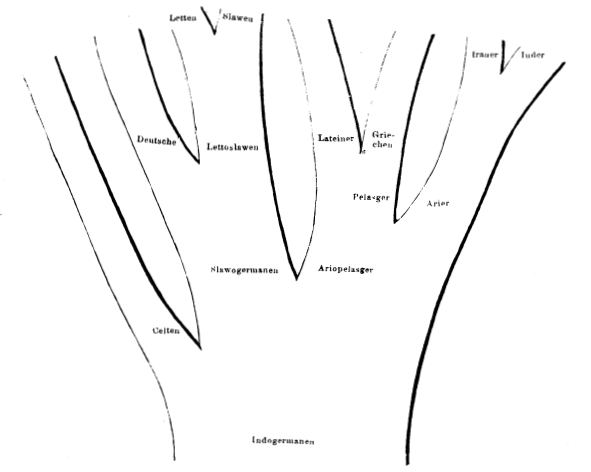
\includegraphics[width=0.5\textwidth]{img/schleicher.jpg}


\subsubsection{\texorpdfstring{{\ldots{} des
Seminarthemas}}{\ldots{} des Seminarthemas}}

\par\noindent\textbf{Die Problematik des Sprachwandels}

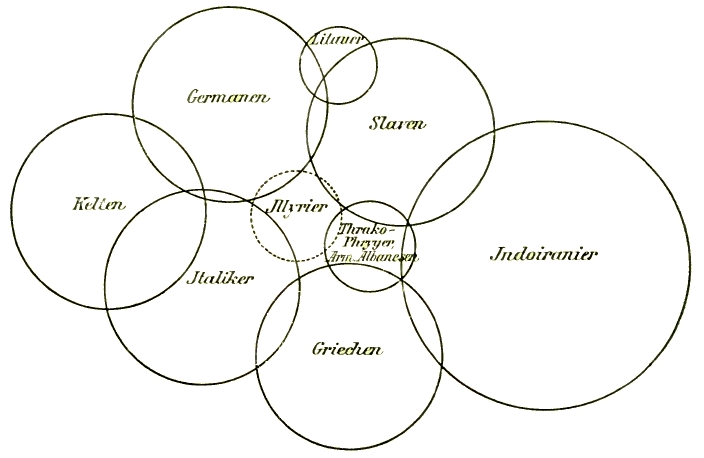
\includegraphics[width=0.5\textwidth]{img/hirt.jpg}
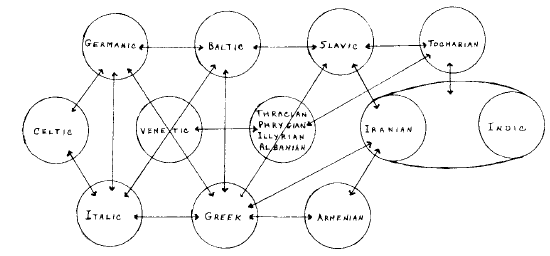
\includegraphics[width=0.5\textwidth]{img/bonfante.png}
\pagebreak


\par\noindent\textbf{Die Wiederentdeckung der Bäume}

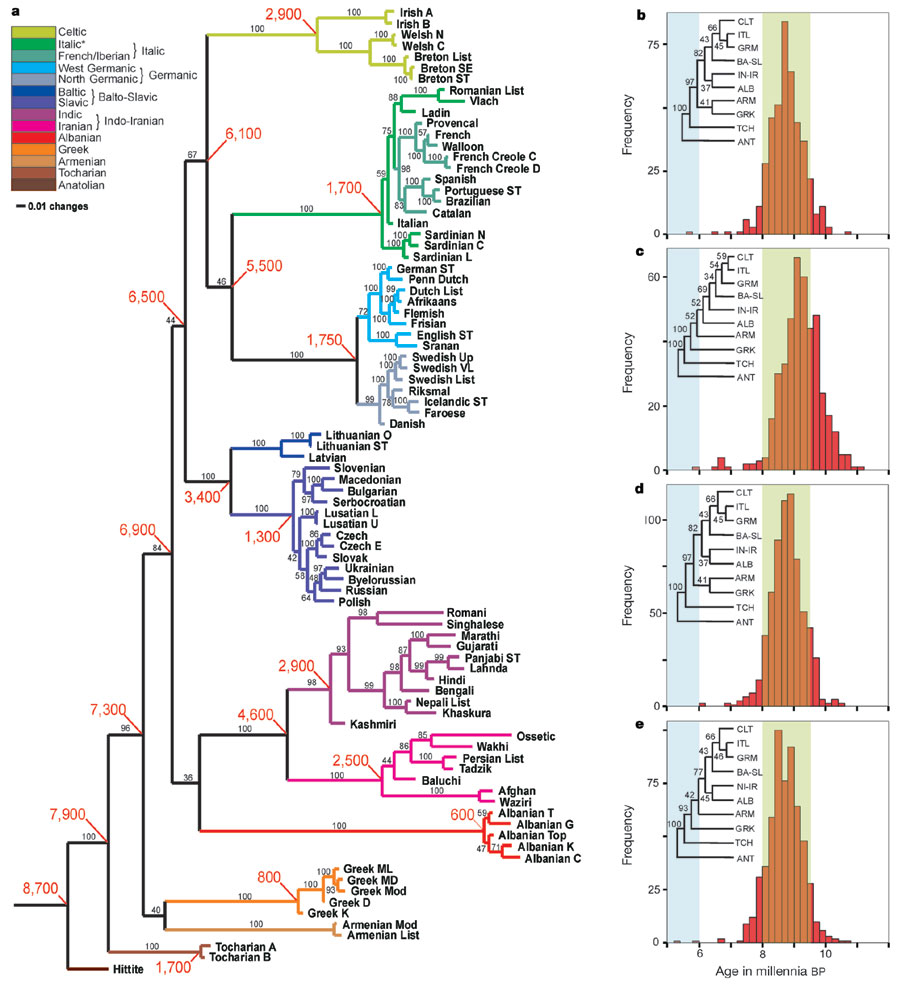
\includegraphics[width=0.5\textwidth]{img/gray.jpg}
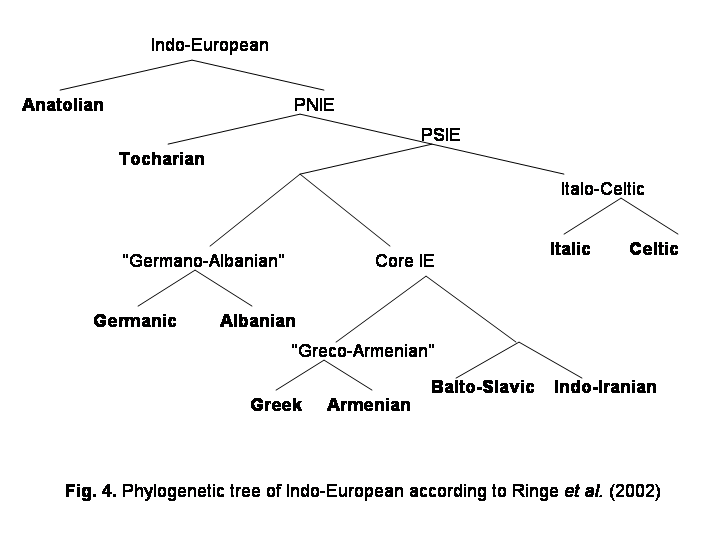
\includegraphics[width=0.5\textwidth]{img/ringe.png}


\includegraphics[width=\textwidth]{img/bridging-1.png}
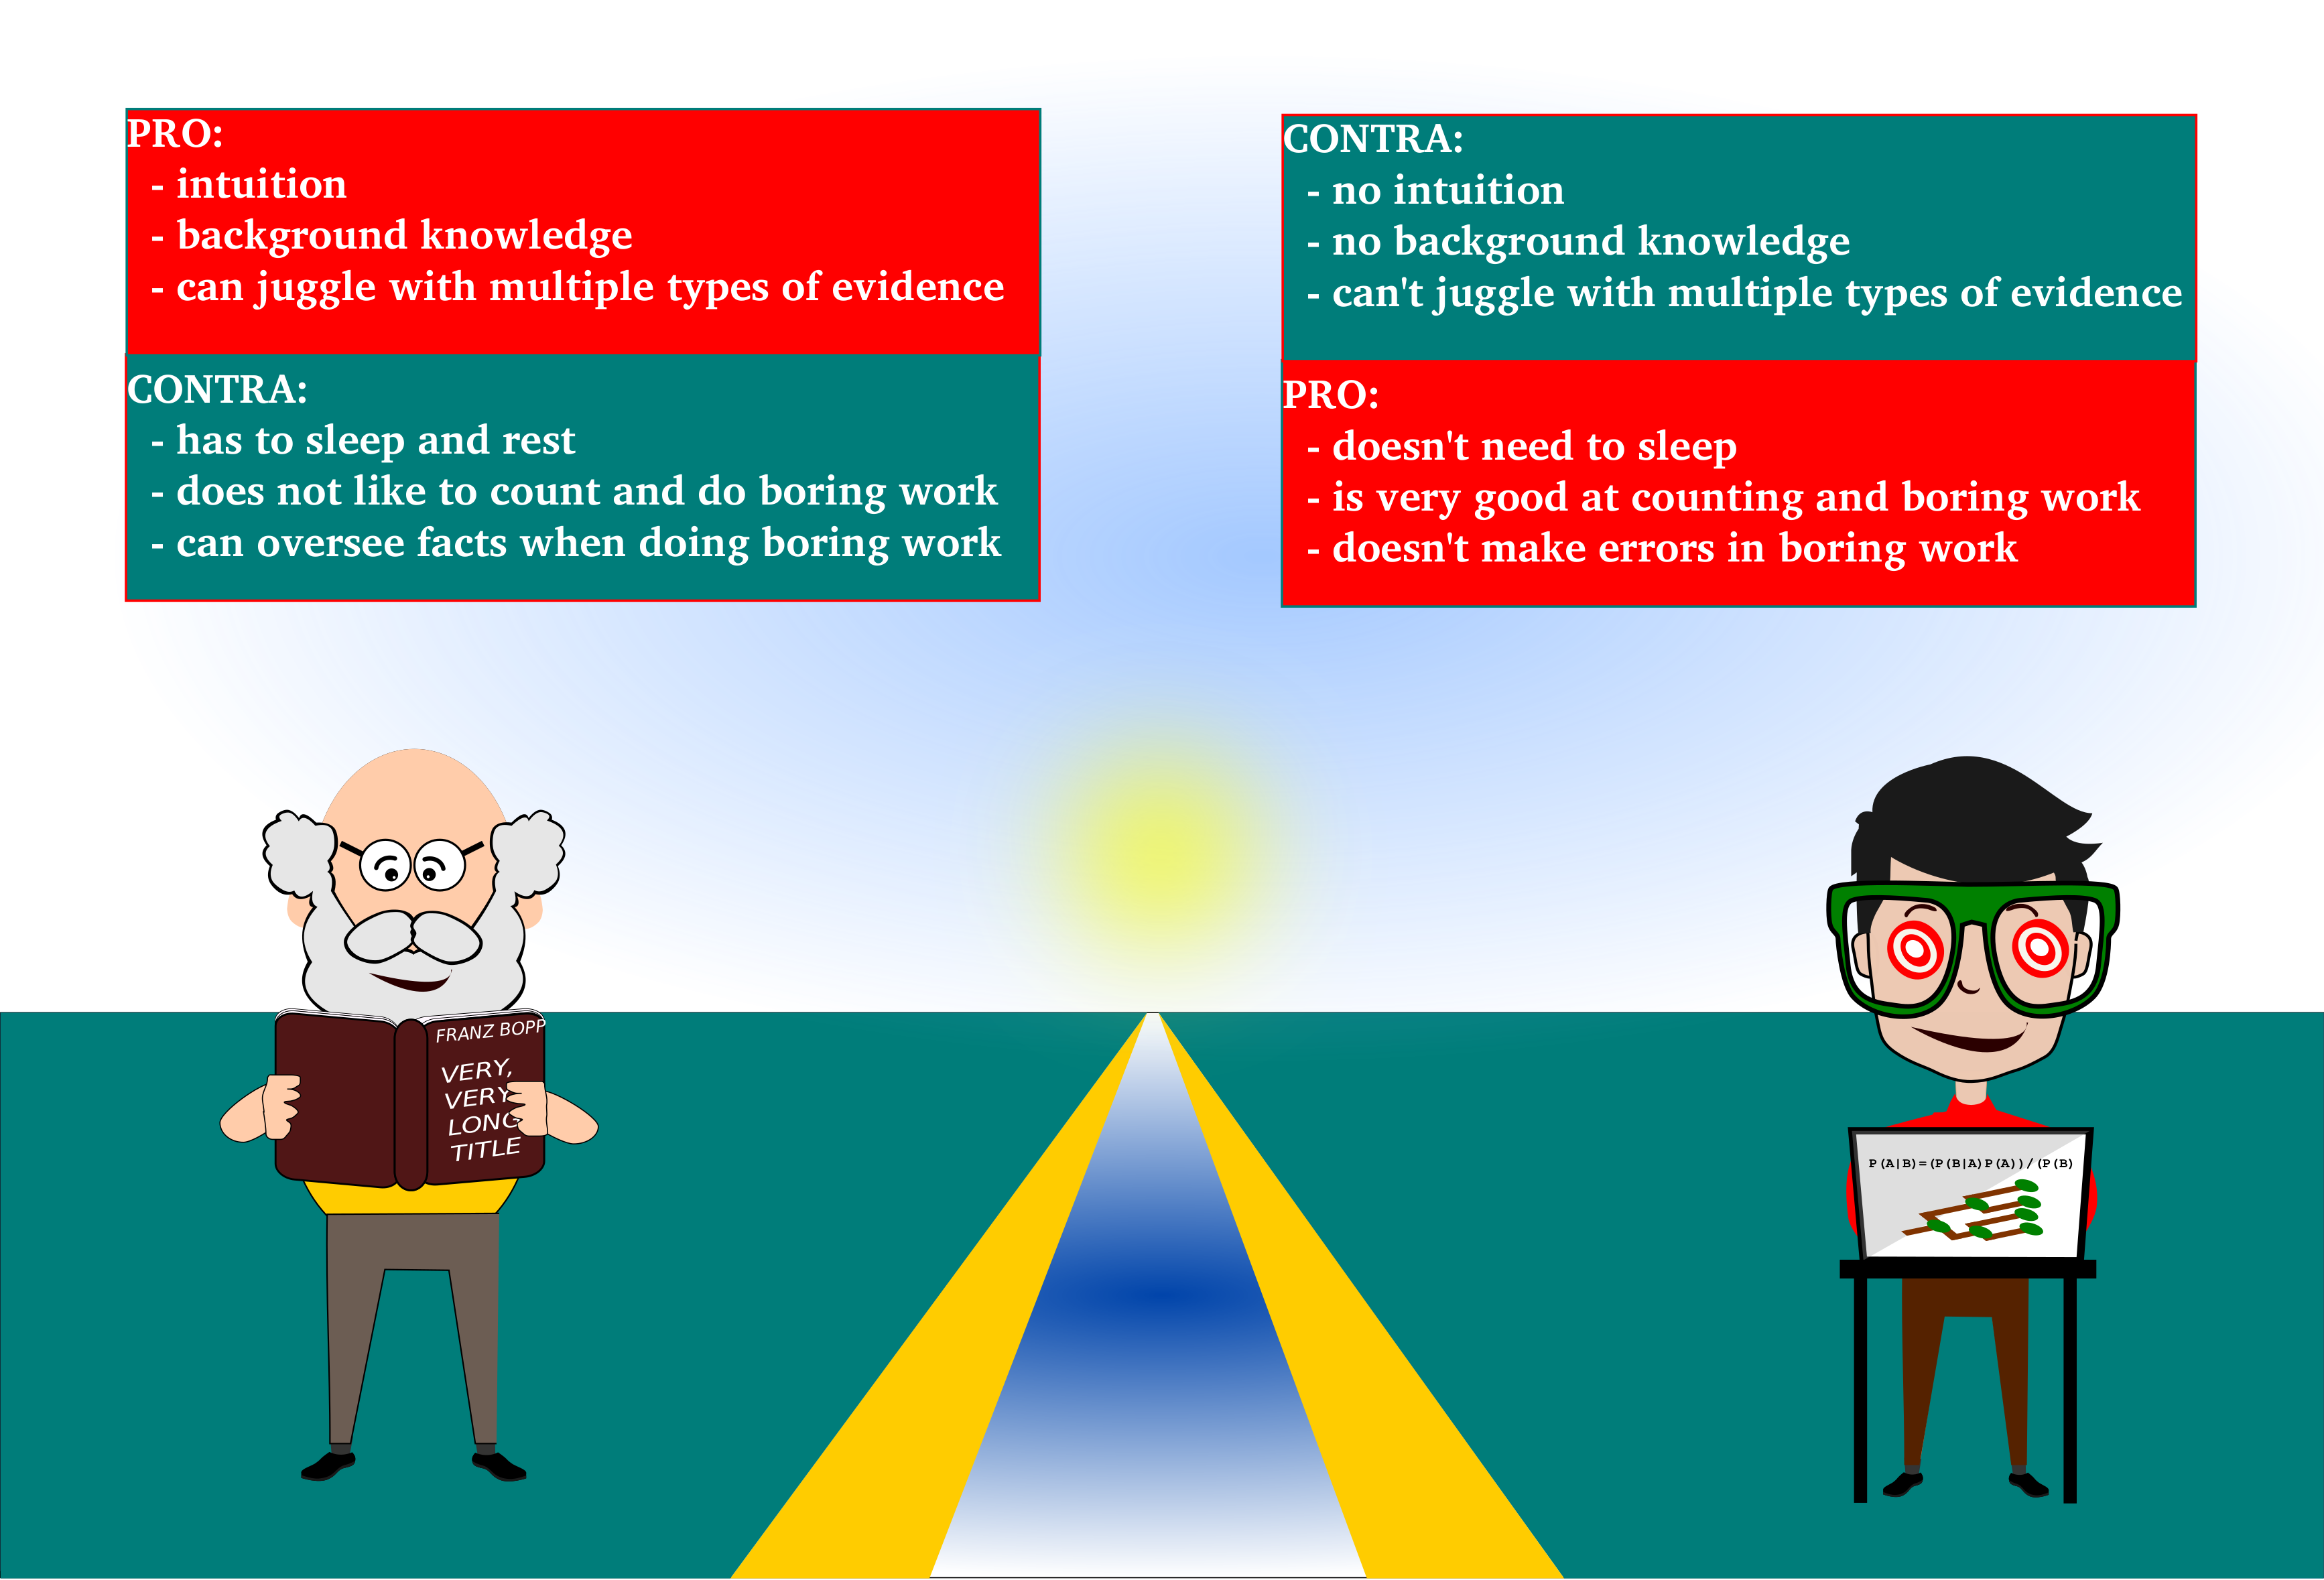
\includegraphics[width=\textwidth]{img/bridging-2.png}

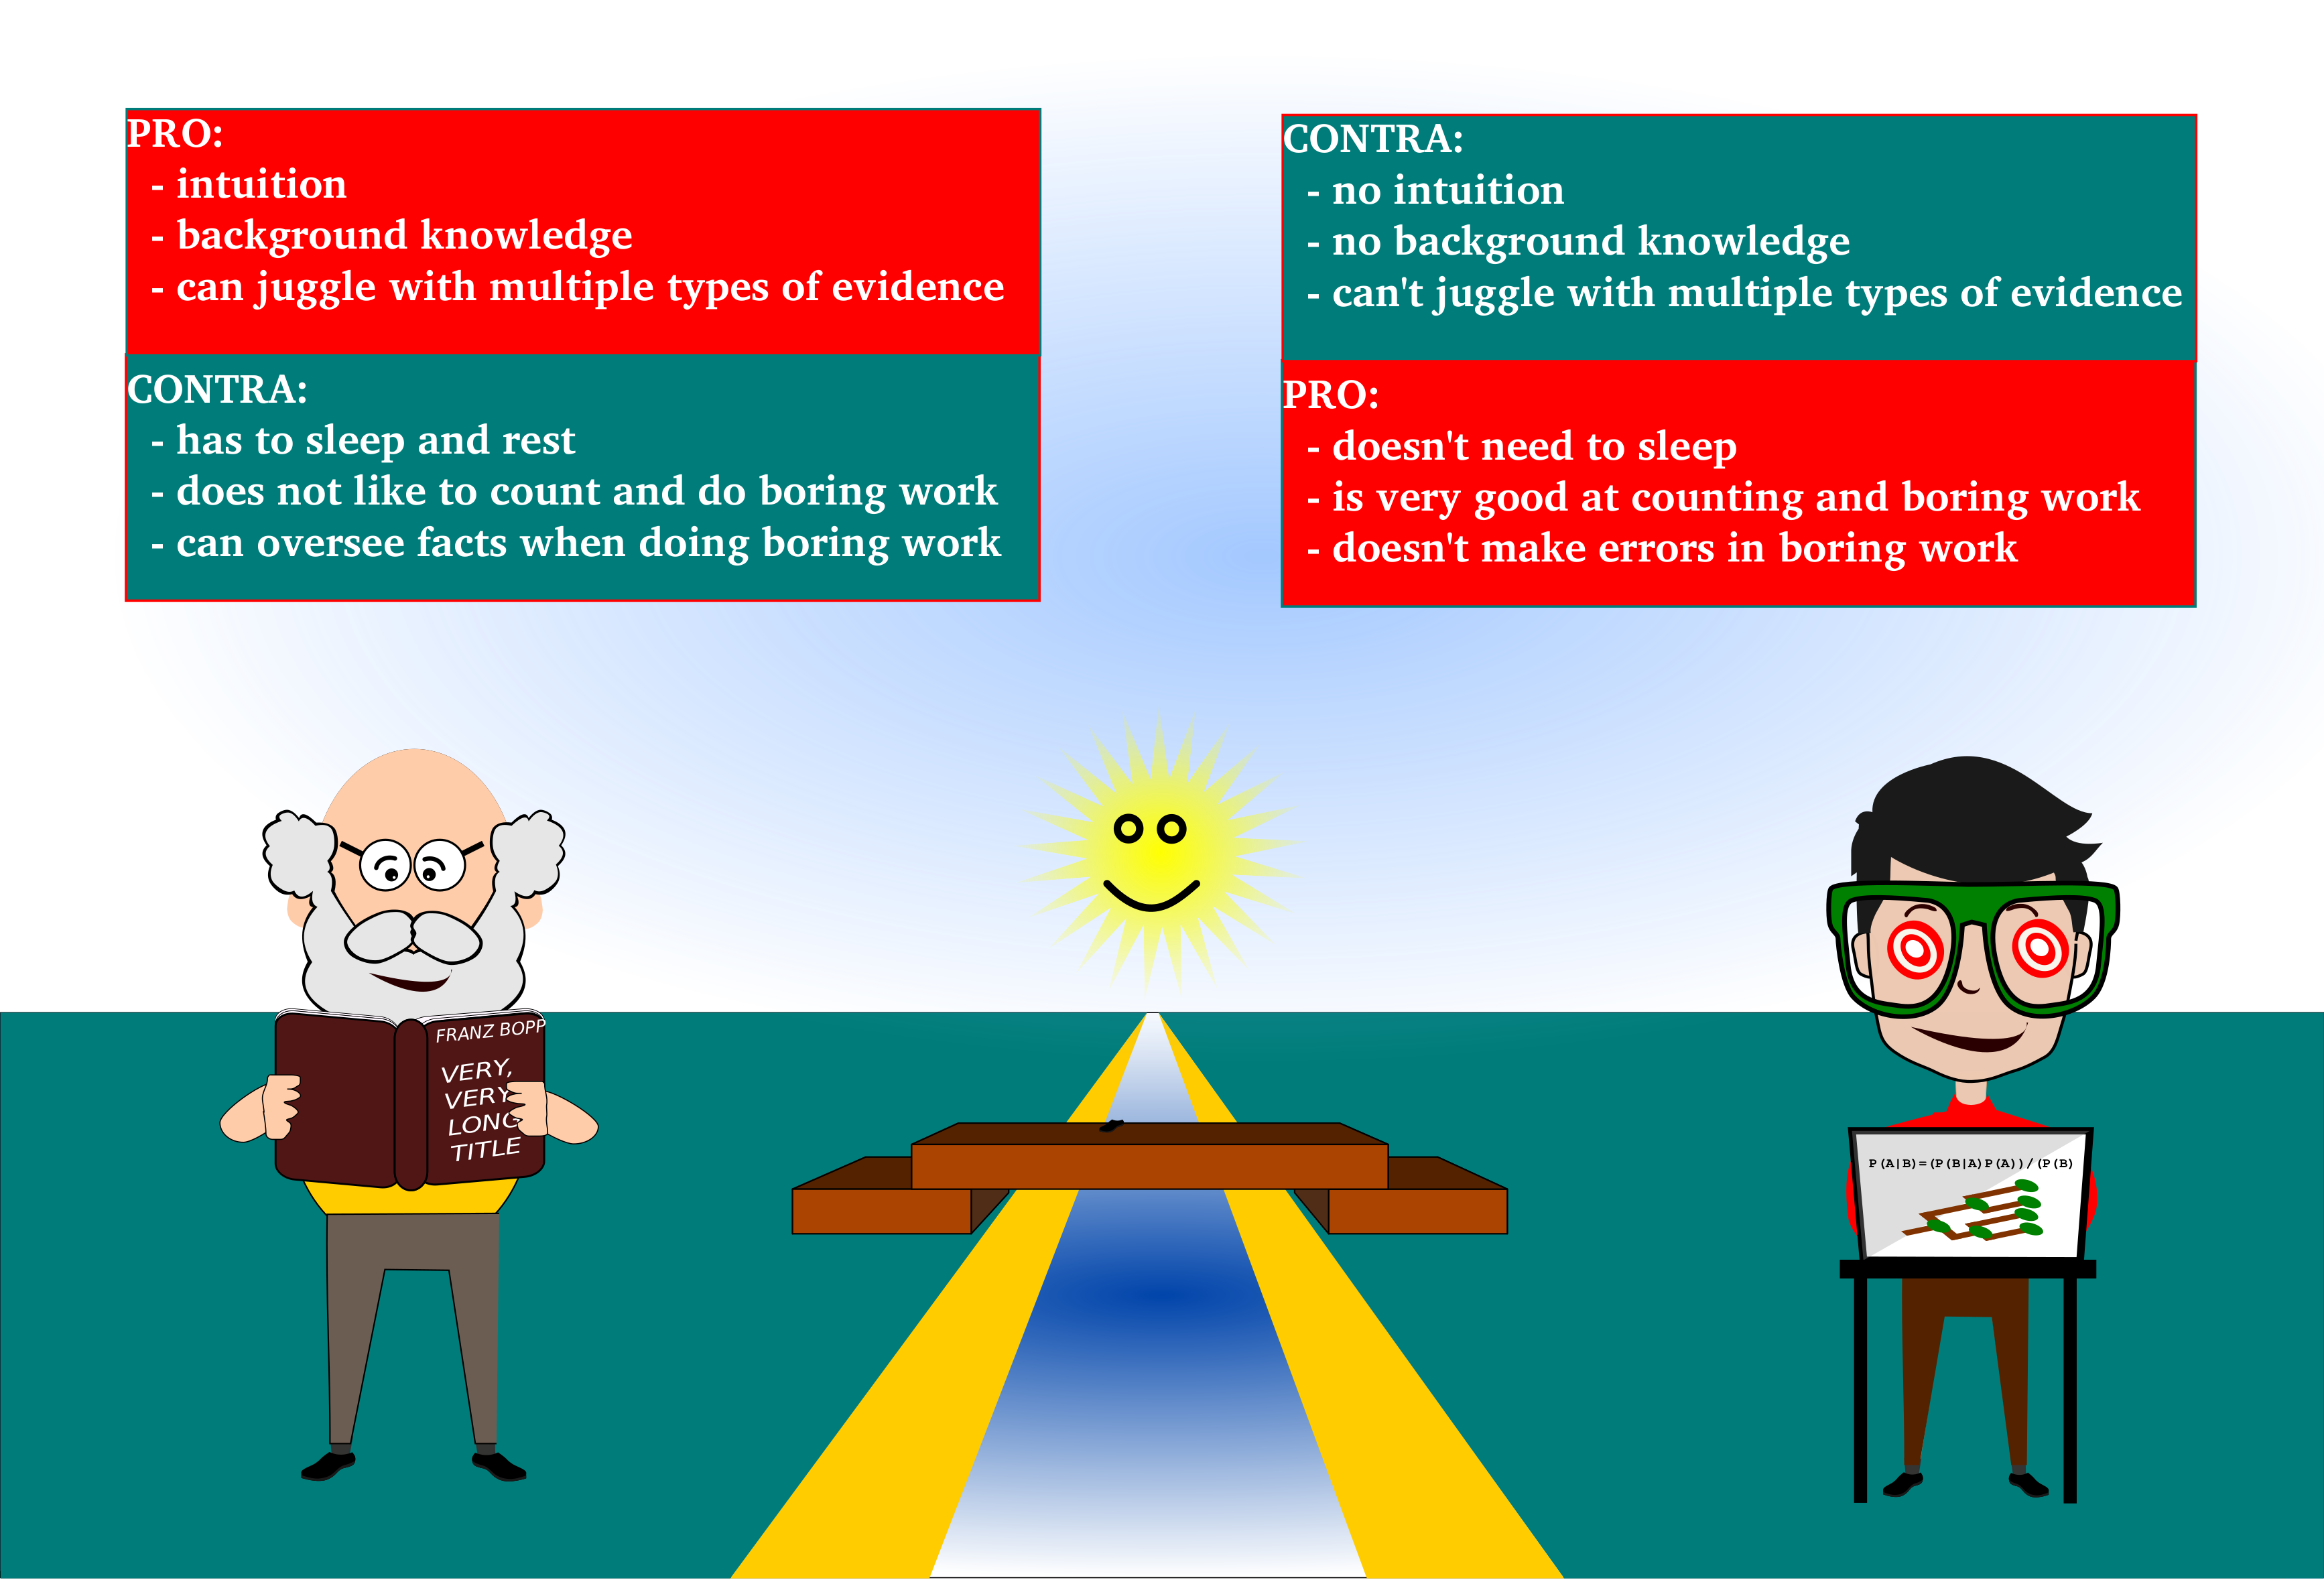
\includegraphics[width=\textwidth]{img/bridging-3.png}
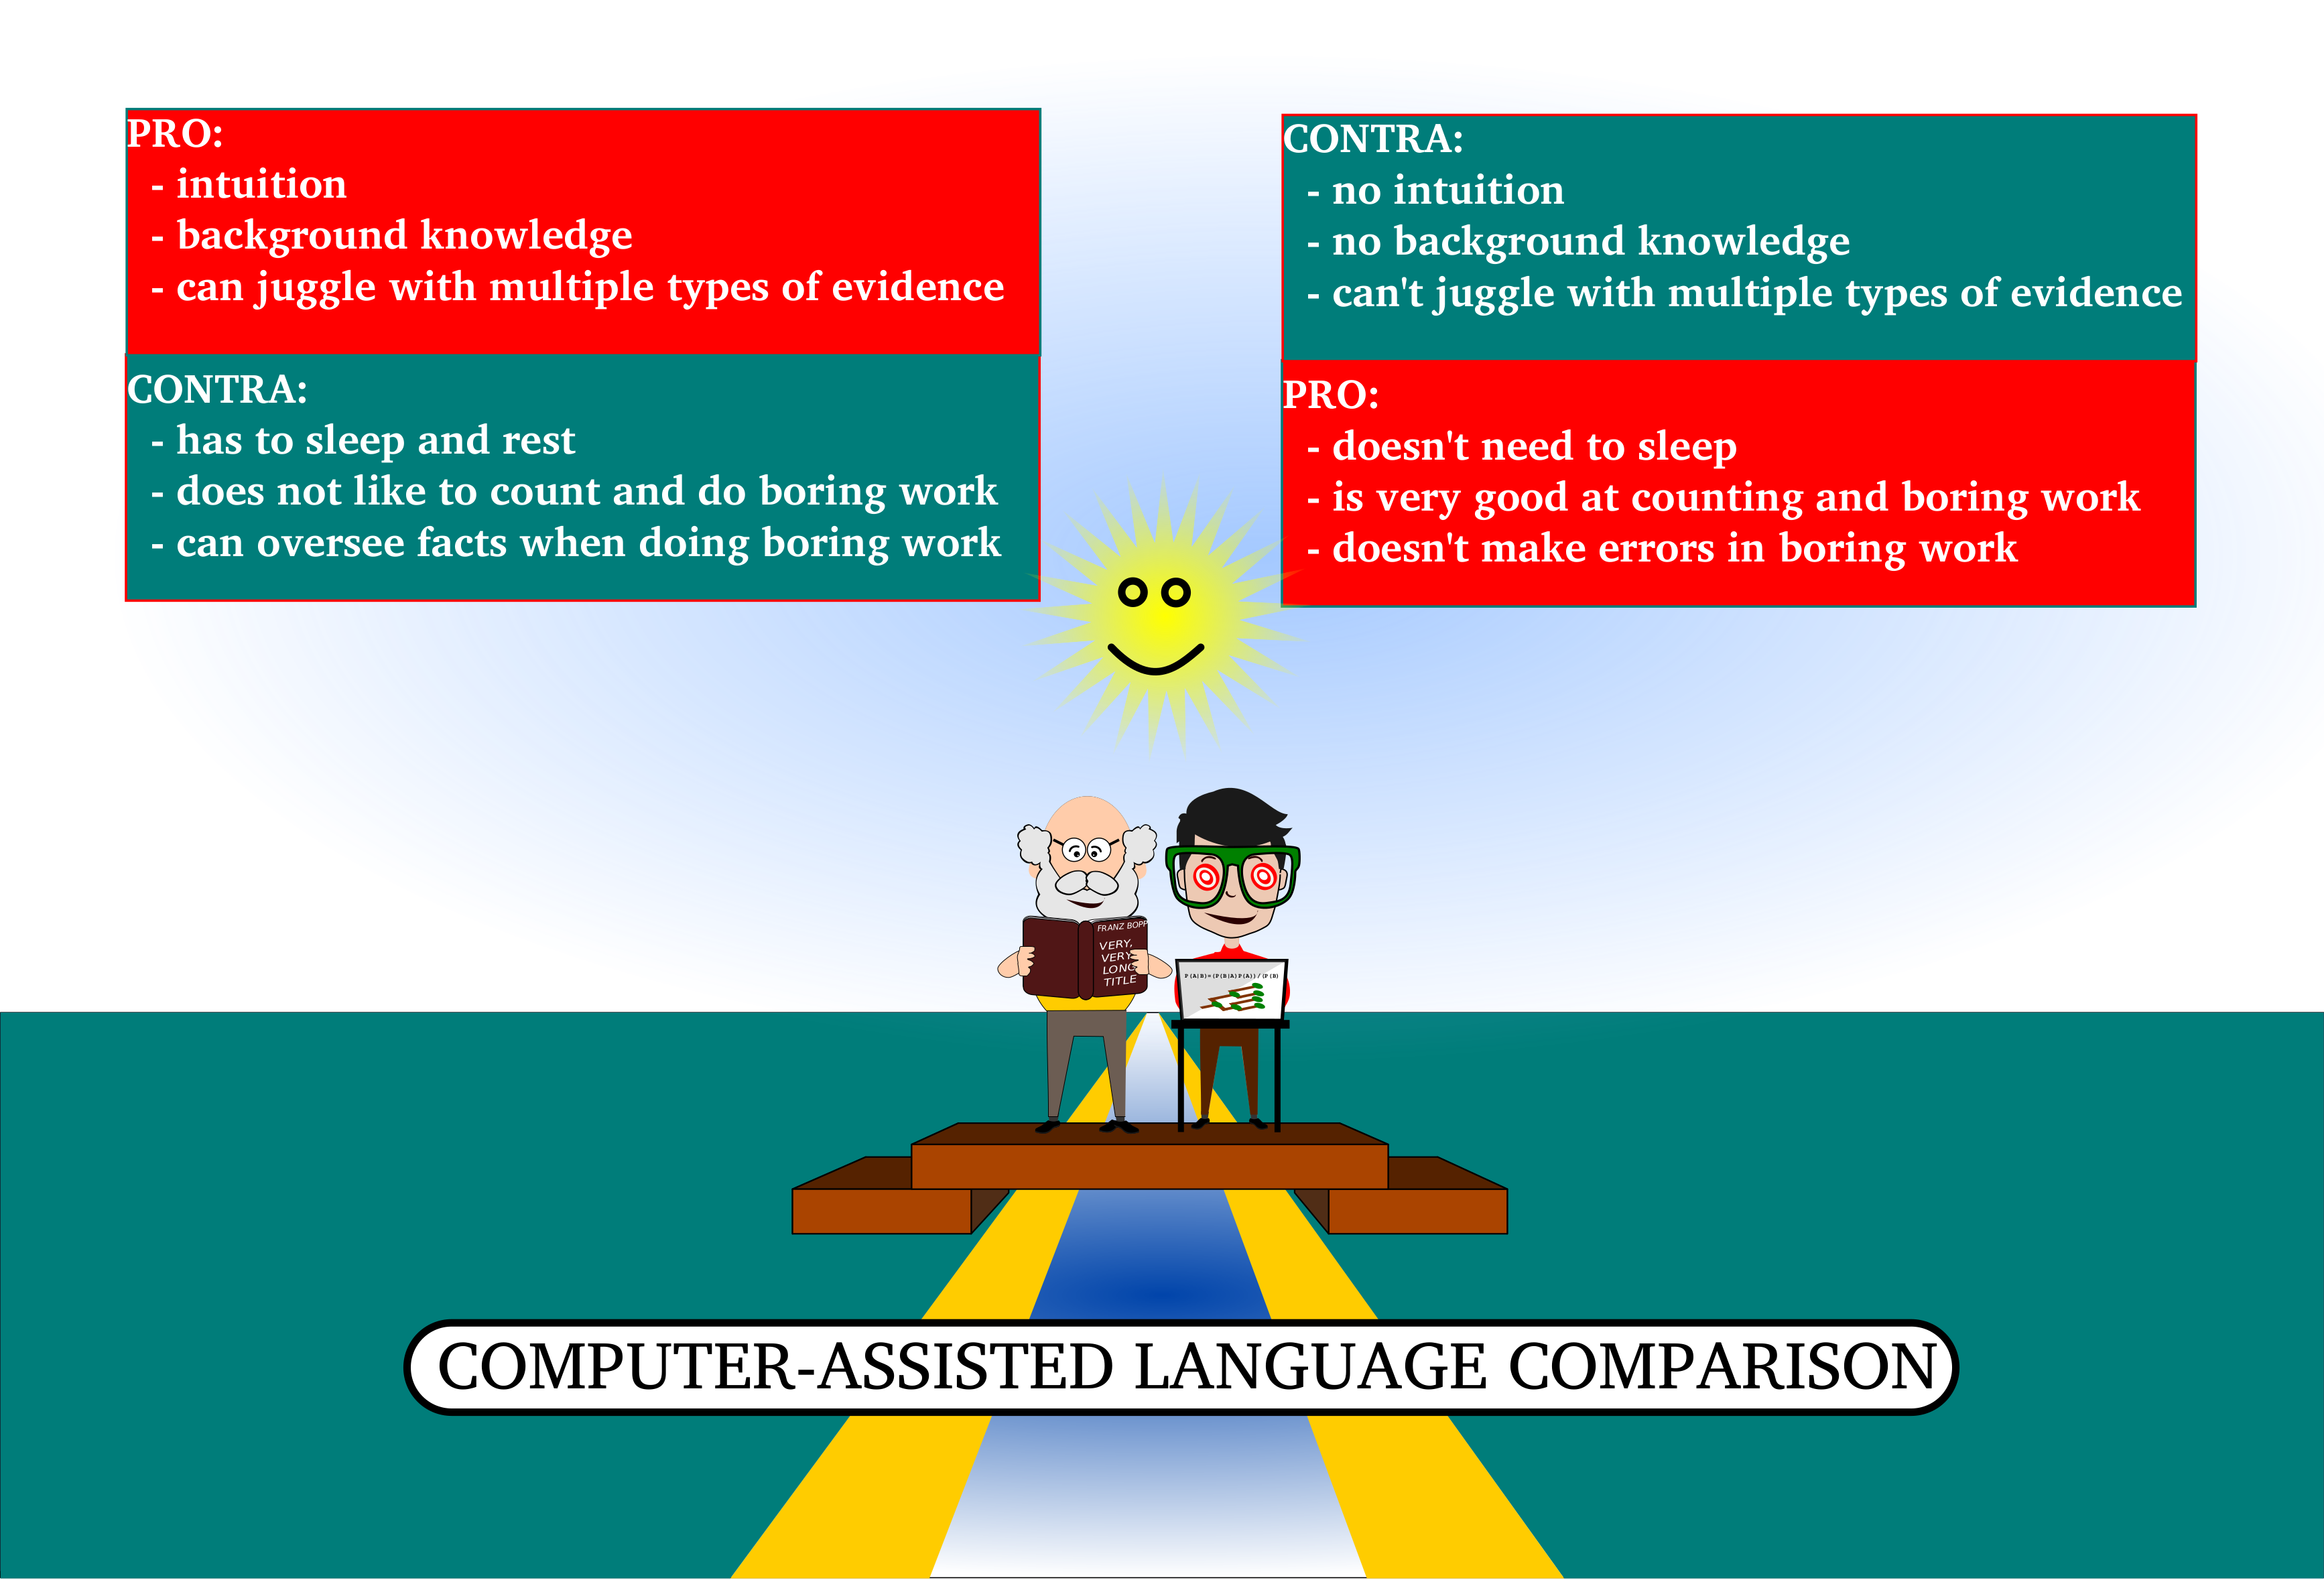
\includegraphics[width=\textwidth]{img/bridging-4.png}
\pagebreak
\par\noindent\textbf{Computergestützter Sprachvergleich}

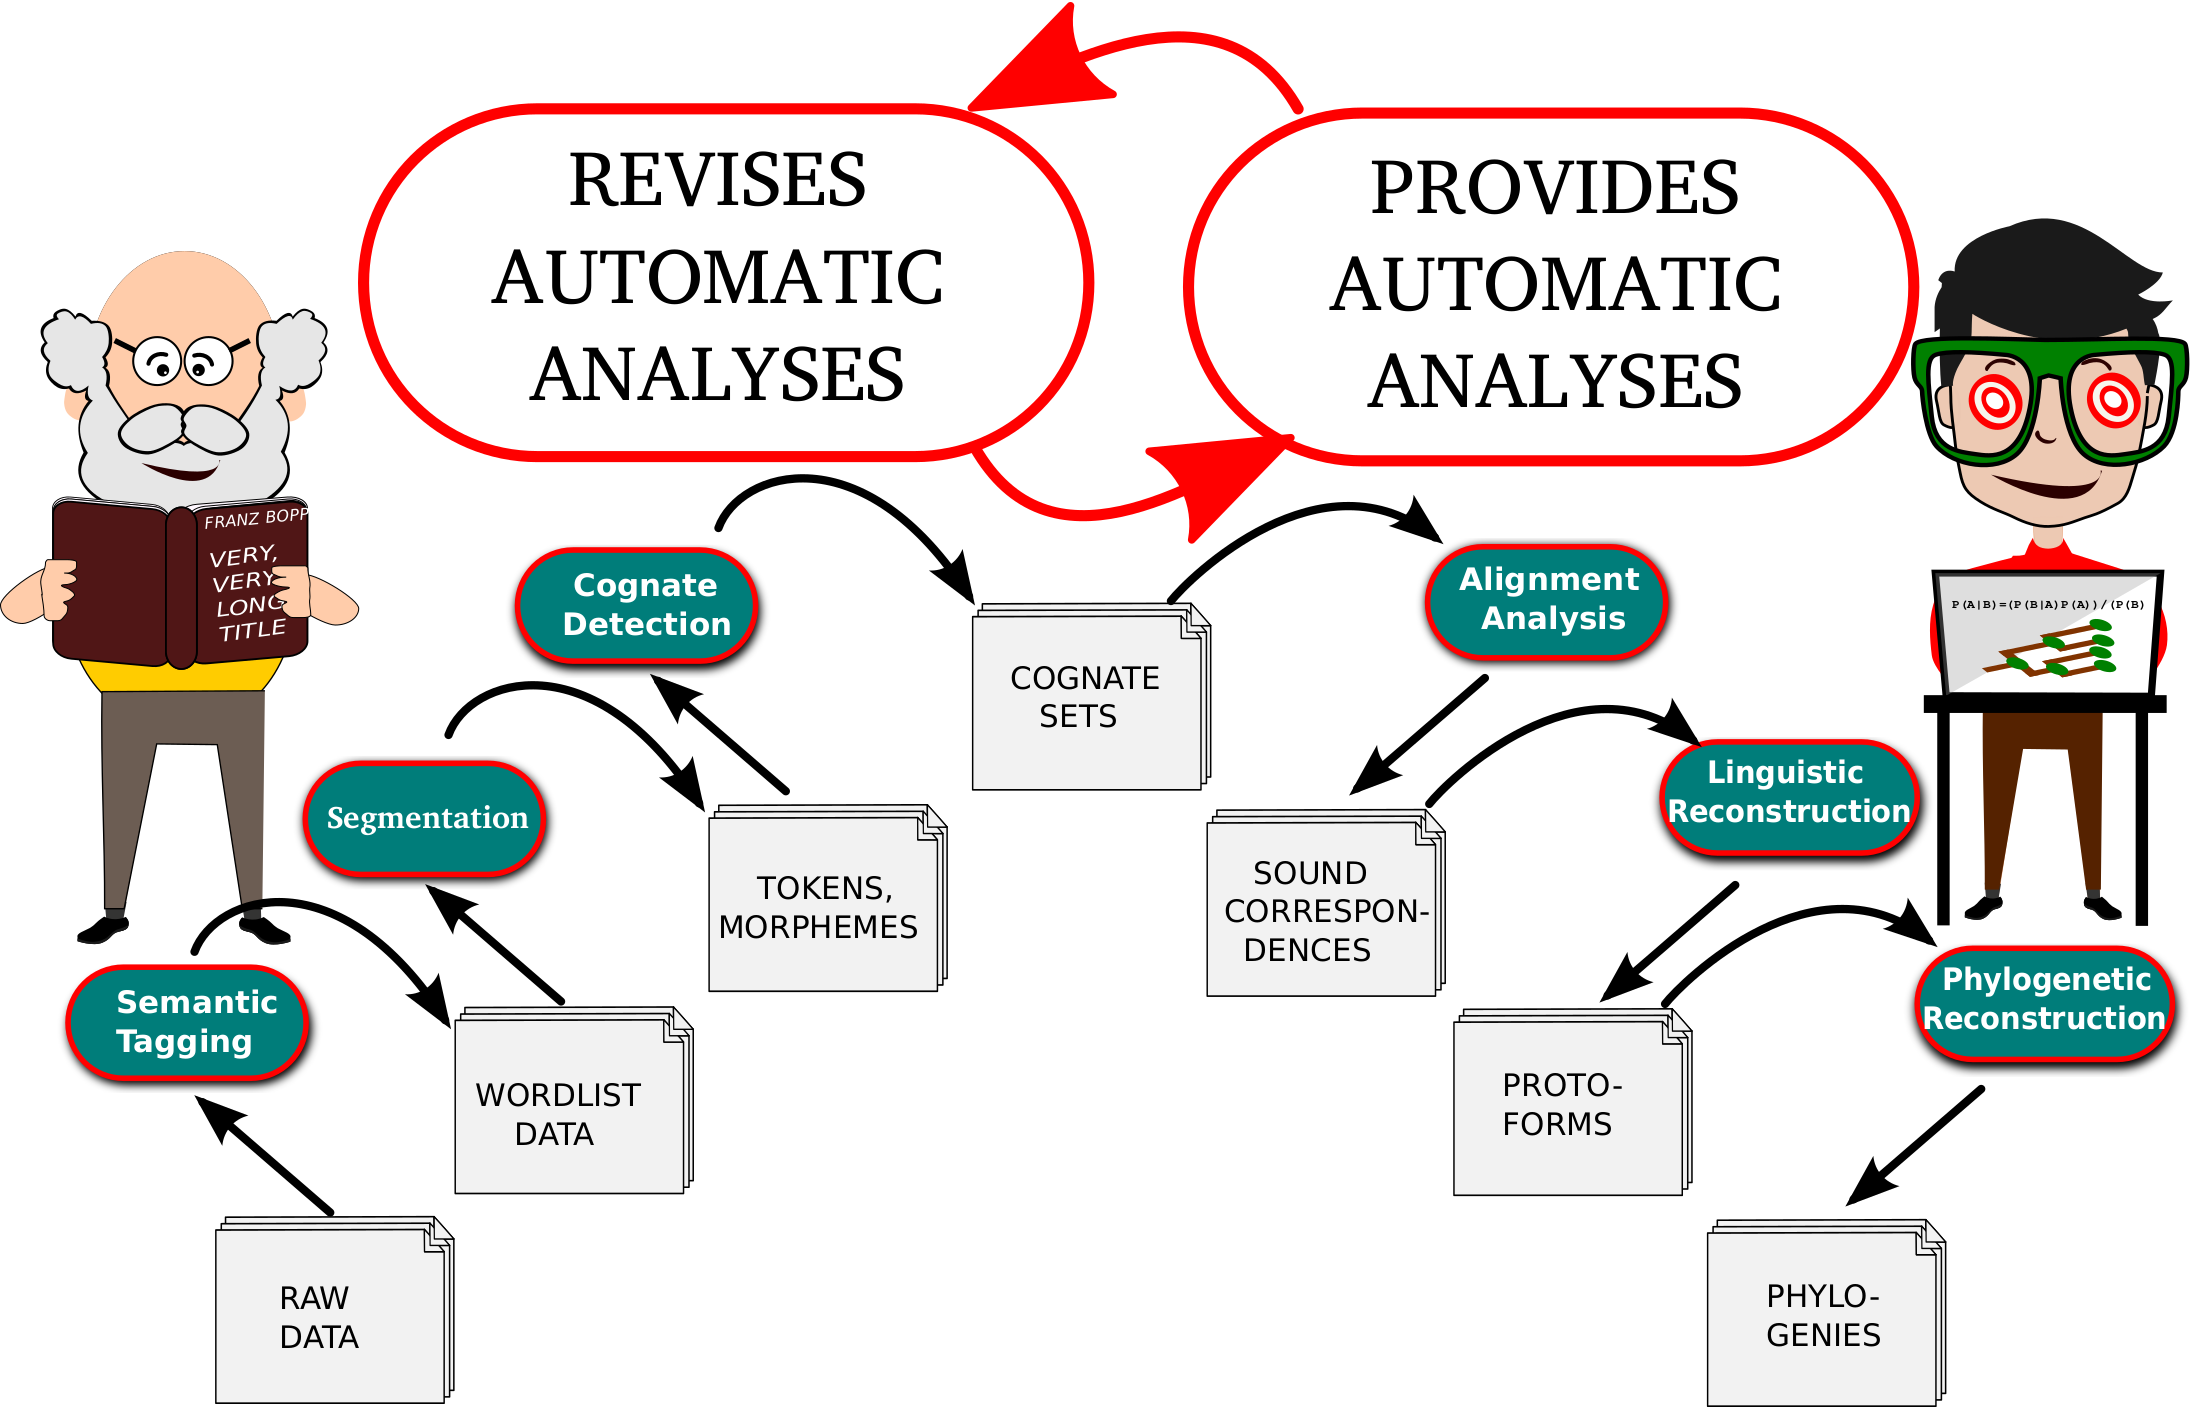
\includegraphics[width=\textwidth]{img/workflows.png}
\subsection{Allgemeines}

\subsubsection{\texorpdfstring{{\ldots{} zum
Programmieren}}{\ldots{} zum Programmieren}}

\par\noindent\textbf{Warum ist es sinnvoll, programmieren zu können?}

{Programmieren zu können ist immer dann sinnvoll, wenn man in seinem
Beruf oder den Studien, denen man nachgeht, häufig wiederholte,
redundante Operationen ausführen muss, die sich ebensogut automatisch
erledigen lassen würden.}



\par\noindent\textbf{Warum ist es sinnvoll, programmieren zu können?}

Wenn man zum Beispiel ein psycholinguistisches Experiment mit 200
Stimuli durchführen will, und wissen möchte, wie häufig die Wörter im
Durchschnitt vorkommen, dann kann man zur Webseite
\url{http://wortschatz.informatik.uni-leipzig.de/} gehen, wo die
Worthäufigkeit für eine Vielzahl von Wörtern verzeichnet ist, und jedes
der Wörter einzeln in das Suchfenster eingeben, um dessen Häufigkeit zu
ermitteln.



\par\noindent\textbf{Warum ist es sinnvoll, programmieren zu können?}

Dies wird dann mindestens zwei Stunden stumpfer Arbeit zur Folge haben,
während der man jedes einzelnen Wort kopiert, die Webseite auf- ruft,
die Häufigkeit kopiert und in eine Tabelle einträgt. Spätestens beim
dritten Experiment, das man durchführt, wird man diese Arbeit hassen und
sich Hiwis wünschen.



\par\noindent\textbf{Daher ist es sinnvoll, programmieren zu können!}

Alternativ kann man auch einfach programmieren: Die Leipziger
Wortschatzprojekt bietet eine Zusatzbibliothek für Python an
(\url{http://pypi.python.org/pypi/libleipzig}), mit deren Hilfe man ganz
schnell ein kleines Programm schreiben kann, das einem für eine
beliebige Liste von Wörtern in Sekundenschnelle alle Frequenzen (und
noch viel mehr Informationen, wenn man will) aus dem Internet
herunterlädt, und --- wenn man will, auch noch den Durchschnitt und die
Standardabweichung aller Frequenzen errechnet.



\par\noindent\textbf{Daher ist es sinnvoll, programmieren zu können!}

Die Eingabe ist dabei denkbar einfach. Um zum Beispiel die absolute
Frequenz des Wortes ``Python'' zu erhalten, muss man auf der
Kommandozeile einfach nur den folgenden Befehl eingeben:

\begin{verbatim}
>>> Frequencies("Python")

[(Anzahl: '129', Frequenzklasse: 17)]
\end{verbatim}


\subsubsection{\texorpdfstring{{\ldots{} zum Programmieren in der
Linguistik}}{\ldots{} zum Programmieren in der Linguistik}}

{ Die Linguistik, insbesondere die historische Linguistik, erlebt
derzeit einen Paradigmenwechsel. Während intuitives umfangreiches
Fachwissen, das Forscher sich über Jahre intensiven Studiums aneignen
mussten, bisher eine sehr große Rolle spielte, und formale Aspekte
lediglich als Gedankenspielereien präsentiert wurden, treten im Rahmen
der Big-Data-Bewegung nun mehr und mehr die empirischen Aspekte der
Disziplin in den Vordergrund. }



Die großen Datensammlungen und die leichte Zugänglichkeit von
Programmiertools machen es zusehends leichter, verschiedenste
Forschungsfragen empirisch zu untersuchen und zu überprüfen. Meiner
Meinung nach ist dies sehr wichtig, da die traditionelle Linguistik sich
viel zu wenig um die Empirie bemüht hat. Es ist jedoch wichtig, sich im
Klaren darüber zu sein, dass eine gute empirische Forschung
\par\noindent\textbf{immer auf den Errungenschaften der traditionellen Linguistik
aufbauen sollte}. Idealerweise praktizieren wir Linguistik als
{computergestützte Forschung}, das heißt, anstelle blind irgendwelchen
Algorithmen zu vertrauen, sollten wir Computermethoden entwickeln, die
helfen, traditionelle Ansätze zu modellieren und hochwertige Datensätze
für die empirische Forschung zu erstellen.

\subsection{Spezielles}

\subsubsection{\texorpdfstring{{\ldots{} zu Algorithmen, Skripten und
Programmen}}{\ldots{} zu Algorithmen, Skripten und Programmen}}

\par\noindent\textbf{Was ist Programmieren?}

\href{http://www.freenetpages.co.uk/hp/alan.gauld/german/tutwhat.htm}{Alan
Gauld} erklärt den Begriff Programmieren wie folgt:

\begin{quote}
Computer-Programmierung ist die Kunst, dass ein Computer das macht, was
du willst.
\end{quote}

{\href{http://de.wikipedia.org/wiki/Computerprogramm}{Wikipedia} ist ein
bisschen ausführlicher:}

\begin{quote}
Ein Computerprogramm oder kurz Programm ist eine Folge von den Regeln
der jeweiligen Programmiersprache genügenden Anweisungen, die auf einem
Computer ausgeführt werden können, um damit eine bestimmte
Funktionalität zur Verfügung zu stellen.
\end{quote}



\par\noindent\textbf{Was ist Programmieren?}

Etymologisch gesehen, bedeutet Programmieren so viel wie ``Vorschriften
erstellen'' und ist im Deutschen laut
\href{http://bibliography.lingpy.org?key=Kluge2002}{Kluge und Seebold
(2002)} zum ersten Mal seit dem 18. Jahrhunder bezeugt.

Entscheidend für das Programmieren, ist, was die Vorschriften betrifft,
dass diese ganz genau befolgt werden, denn so ergibt sich die
Möglichkeit, egal, ob das Programm nun von einem Menschen oder einem
Computer ausgeführt wird, dass das gewünschte Ergebnis immer erzielt
wird.



\par\noindent\textbf{Was ist ein Algorithmus?}

{Im \href{http://bibliography.lingpy.org?key=Kluge2002}{Kluge} finden
wir die Folgende Definition:}

\begin{quote}
\par\noindent\textbf{Algorithmus.} Substantiv Maskulinum, ``Berechnungsverfahren'',
peripherer Wortschatz, fachsprachlich (13. Jh., Form 16. Jh.), mhd.
algorismus. Onomastische Bildung. Entlehnt aus ml. algorismus, das das
Rechnen im dekadischen Zahlensystem und dann die Grund- rechenarten
bezeichnet. Das Wort geht zurück auf den Beinamen Al-Hwārizmī (''der
Chwa- resmier'', eine Herkunftsbezeichnung) eines arabischen
Mathematikers des 9. Jhs., durch dessen Lehrbuch die (indischen und
dann) arabischen Ziffern in Europa allgemein bekannt wurden. Das
Original des hier in Frage kommendes Buches ist verschollen, die ml.
Über- setzung ist Liber algorismi de practica arismetrice. Die
Schreibung mit

in Anlehnung an gr. arithmós ``Zahl''. {[}\ldots{}{]}
\end{quote}



\par\noindent\textbf{Was ist ein Algorithmus?}

{\href{http://bibliography.lingpy.org?key=Brassard1993}{Brassard und
Bratley (1993)} sind da weniger etymologisch:}

\begin{quote}
Das Concise Oxford Dictionary definiert einen Algorithmus als
``Verfahren oder Regeln für (speziell maschinelle) Berechnung''. Die
Ausführung eines Algorithmus darf weder sub- jektive Entscheidungen
beinhalten noch unsere Intuition und Kreativität fordern. Wenn wir über
Algorithmen sprechen, denken wir meistens an Computer.
Nichtsdestoweniger könn- ten andere systematische Methoden zur Lösung
von Aufgaben eingeschlossen werden. So sind zum Beispiel die Methoden
der Multiplikation und Division ganzer Zahlen, {[}\ldots{}{]} ebenfalls
Algorithmen. {[}\ldots{}{]} Es ist sogar möglich, bestimmte Kochrezepte
als Algorithmen aufzufassen, vorausgesetzt, sie enthalten keine
Anweisungen wie ``nach Geschmack salzen''.
\end{quote}



\begin{itemize}
\itemsep1pt\parskip0pt\parsep0pt
\item
  Ein Algorithmus ist eine geordnete Sammlung von Verfahren, mit deren
  Hilfe eine Aufgabe (ein Problem) eindeutig gelöst werden kann.
\item
  Ein Programm ist eine \emph{Implementierung} von Algorithmen mit Hilfe
  einer speziellen Programmiersprache.
\item
  Ein Skript ist ein Programm, das in einer interpretierten
  Programmiersprache (einer Skriptsprache) geschrieben wurde. Alle
  Programme, die mit Python oder JavaScript erstellt werden, sind
  demnach Skripte.
\end{itemize}


\subsubsection{\texorpdfstring{{\ldots{} zur Grundausstattung fürs
Programmieren}}{\ldots{} zur Grundausstattung fürs Programmieren}}

\par\noindent\textbf{Texteditoren}

Um Skripte zu schreiben, benötigen wir einen guten
\href{http://de.wikipedia.org/wiki/Texteditor}{Texteditor}. Das ist
nicht das gleiche wie Word oder LibreOffice, sondern ein Editor, der
reinen Text schreibt. Aus Zeitgründen erwarte ich von allen Teilnehmern
des Seminars, dass sie sich eigenständig einen guten Texteditor zulegen,
um Skripte zu schreiben. Ferner ist zu beachten, dass alle Dateien in
\href{https://de.wikipedia.org/wiki/UTF-8}{UTF-8} abgespeichert werden
solltet.

Ich selbst schreibe meine Skripte alle mit \href{http://vim.org}{VIM}.
Weitere populäre Texteditoren sind:

\begin{itemize}
\itemsep1pt\parskip0pt\parsep0pt
\item
  \href{https://www.gnu.org/software/emacs/}{GNU Emacs}: der natürliche
  Feind von allen, die gerne VIM benutzen
\item
  \href{http://de.wikipedia.org/wiki/Notepad++}{Notepad++}: ein relativ
  ordentlicher Texteditor für Windows-Benutzer
\end{itemize}



\par\noindent\textbf{Versionsverwaltungssoftware}

Wer größere Projekte schreibt, kommt ohne sie nicht aus: die Software
zur Versionsverwaltung. Ich selbst verwende
\href{http://de.wikipedia.org/wiki/Git}{Git} für meine Arbeit, da es
sich wunderbar mit \href{http://github.org}{GitHub} integrieren lässt,
und Daten dadurch auch anderen Nutzern zur Verfügung gestellt werden
können. Für das Seminar setze ich voraus, dass jeder Teilnehmer sich
grundlegend mit den Ideen hinter Git auseinandersetzt. Um an bestimmte
Resourcen zu gelangen, die ich anbiete, wird ferner ein GitHub Account
benötigt werden. Ich empfehle ohnehin allen Programmierinteressierten,
sich einen GitHub Account anzulegen, da sich GitHub mehr und mehr zum
Standard für kollaboratives Arbeiten entwickelt (was nicht heißt, dass
ich es gut finde, dass dahinter ein Konzern steckt!).



\par\noindent\textbf{Möglichkeiten zum Datenhosting}

Wer als Linguist programmiert möchte irgendwann auch seinen Sourcecode
anderen Nutzern zur Verfügung stellen. Das ist sehr leicht möglich mit
Hilfe neuer gemeinnütziger Anbieter. Ich empfehle in diesem Zusammenhang
\href{http://zenodo.org}{Zenodo}. Man kann sich mit seinem GitHub
Account anmelden, und seinen Code entweder automatisch von Zenodo hosten
lassen, oder ihn direkt manuell hochladen. Zenodo garantiert
Langzeitarchivierung, ist kostenlos (weil gemeinnützig), und erlaubt bis
zu zwei Gigabyte an Daten pro Projekt. Außerdem bekommt man von Zenodo
immer automatisch einen
\href{http://de.wikipedia.org/wiki/Digital_Object_Identifier}{Digital
Object Identifier}, was gewährleistet, dass die Daten im Netz auffindbar
und unmissverständlich referenzierbar sind.


\subsubsection{\texorpdfstring{{\ldots{} zu Python und
JavaScript}}{\ldots{} zu Python und JavaScript}}

\par\noindent\textbf{Vorzüge von Python (frei nach
\href{http://bibliography.lingpy.org?key=Bassi2010}{Bassi (2010:10)})}

\begin{itemize}
\itemsep1pt\parskip0pt\parsep0pt
\item
  \textbf{Readability}: Python is a ``human-readable language''
\item
  \textbf{Built-in features}: Python comes with ``batteries included''
\item
  \textbf{Availability of third-party modules}: plotting, game
  development, databases, etc. to model real-world data
\item
  \textbf{multi-paradigm}: can be used as a procedural and
  object-oriented programming language
\item
  \textbf{extensibility}: Python can be connected to many other
  languages
\item
  \textbf{open source}: liberal open source license, also for commercial
  use
\item
  \textbf{cross-platform}: works on any computer (even Windows)
\item
  \textbf{thriving community}: ask whatever question on
  \href{http://stackoverflow.com}{stackoverflow}, you'll get an answer
  in most of the cases
\end{itemize}



\par\noindent\textbf{Vorzüge von JavaScript (frei nach Meinung von mir)}

\begin{itemize}
\itemsep1pt\parskip0pt\parsep0pt
\item
  \textbf{cross-platform}: JavaScript ist die einzig wirkliche
  Cross-Platformsprache, weil jeder, der einen Webbrowser hat, sie auch
  hat
\item
  \textbf{schön anzusehen}: JavaScript ist sehr hilfreich, wenn man
  Programme schreiben will, die optisch ansprechend sind
\item
  \textbf{leicht zu verwenden (für den Anwender)}: JavaScript macht es
  dem Anwender leicht (dem Programmierer aber leider eher schwer)
\item
  \textbf{Schönheit ist nicht alles}: JavaScript ist eine durchweg
  hässliche Sprache. Dennoch kann man sich mit ihr ganz ordentlich
  arrangieren.
\item
  \textbf{große Unterstützergemeinschaft}: wahrscheinlich sogar größer
  als die von Python: man findet sehr schnell antworten zu Fragen im Web
\item
  \textbf{viele Third-Party-Modules}: es gibt eine Unmenge von Modulen,
  auf die man zurückgreifen kann, und noch viel mehr kurze Beispiele
\end{itemize}



Mit Python und JavaScript hat man zwei unheimlich Mächtige Tools zur
Hand, die es einem erlauben, Daten nicht nur auf hochwertige Weise zu
analysieren, sondern die Ergebnisse auch noch interaktiv zu
präsentieren. Für die moderne, computergestützte Wissenschaft, ist es
ein großer Vorteil, über Grundwissen in beiden Sprachen zu verfügen.


